\FloatBarrier
\section{A worked example: one, two and three hosts}\label{sec:example}

Before turning to the general derivations, we compare life cycles with one, two, and three hosts in the linear, rare-parasite ring model of Section~\ref{sec:model} (Eq.~\eqref{eq:model-ring}). All parameter values here are illustrative choices in that model rather than measurements on a specific species. Take one month as the time step (results hold in units of the step). Each mean model is calibrated to $R_0 = \lambda = 1$ (the invasion threshold without fluctuations, where $R_0$ is the baseline expected descendants completing one cycle and $\lambda$ is the mean-matrix per-step growth factor), with memoryless geometric stage stays of mean $\tau_k$ months, staying fractions $1 - 1/\tau_k$, mean transfers $1/\tau_k$, and mean generation time $\mathcal{T} = \sum_{k=1}^n \tau_k$ across the $n$ stages. The parasite spends a mean stay of $a = 6$ months in the one stage whose outward transfer depends on a fluctuating host, while every other host is a steady stage (constant host multiplier $h_k(t) \equiv 1$). That host's abundance, scaled to an arithmetic mean of one, has a logarithm that follows a Gaussian first-order autoregressive process with standard deviation $\sigma$ (variance $\sigma^2$) and monthly lag-one correlation $\phi$ (Eq.~\eqref{eq:model-ar1}). Writing $\theta = \phi/(1 - \phi)$ for the host memory scale (in months), we compare uncorrelated monthly host numbers ($\phi = 0$, $\theta = 0$) with multi-month booms and busts ($\phi = 0.8$, $\theta = 4$ months).

Here $\Gamma$ (Proposition~\ref{prop:ring-gamma}, Eq.~\eqref{eq:ring-gamma}) is the quadratic (second-order, meaning the leading effect of small fluctuations, proportional to $\sigma^2$) approximation to the threshold loss $D$ in $\ln R_0$ (Eq.~\eqref{eq:model-loss}, Proposition~\ref{prop:bounds-r0star}). A rare parasite invades only if $\ln R_0$ exceeds $D$, so a relative loss of $2$ means fluctuations raise the invasion hurdle twice as much as in the one-host cycle of stay $a = 6$ months, where $\Gamma/\sigma^2 = 1/(2a) = 1/12 \approx 0.08333$ at every $\phi$ (Proposition~\ref{prop:ring-band}).

\begin{table}[htbp]
\caption{Fluctuation loss across illustrative one-, two-, and three-host life cycles in series and across alternative hosts in parallel$^{\mathrm{a,b}}$}\label{tab:example}
{\footnotesize\setlength{\tabcolsep}{4pt}
\begin{tabular*}{\textwidth}{@{\extracolsep{\fill}}lrrrrr@{}}
\toprule
\multicolumn{6}{@{}l@{}}{\textit{Part A. Obligate hosts in series (fluctuating stay $a = 6$ months)}} \\
\addlinespace[2pt]
 & & \multicolumn{2}{c}{Autocorrelated ($\phi = 0.8$)} & \multicolumn{2}{c}{Uncorrelated ($\phi = 0$)} \\
\cmidrule(lr){3-4}\cmidrule(lr){5-6}
Life cycle & $\mathcal{T}$ (mo) & $\Gamma/\sigma^2$ & Relative & $\Gamma/\sigma^2$ & Relative \\
\midrule
1 host (no steady stage) & $6$ & $0.08333$ & $1.00$ & $0.08333$ & $1.00$ \\
2 hosts, steady stay $3$ & $9$ & $0.20370$ & $2.44$ & $0.05556$ & $0.67$ \\
2 hosts, steady stay $60$ & $66$ & $0.04254$ & $0.51$ & $0.00758$ & $0.091$ \\
3 hosts, steady stays $30 + 30$ & $66$ & $0.06261$ & $0.75$ & $0.00758$ & $0.091$ \\
3 hosts, steady stays $1 + 59$ & $66$ & $0.04744$ & $0.57$ & $0.00758$ & $0.091$ \\
\bottomrule
\end{tabular*}
\par\vspace{3pt}
\begin{tabular*}{\textwidth}{@{\extracolsep{\fill}}lrr@{}}
\toprule
\multicolumn{3}{@{}l@{}}{\textit{Part B. Equal-share matched alternative hosts in parallel (stays $6$ and $24$ months, $\mathcal{T} = 30$)}} \\
\addlinespace[2pt]
Alternative hosts $M$ & Relative loss, independent ($\rho = 0$) & Relative loss, perfectly synchronous ($\rho = 1$) \\
\midrule
$1$ & $1.00$ & $1.00$ \\
$2$ & $0.50$ & $1.00$ \\
$3$ & $0.33$ & $1.00$ \\
$4$ & $0.25$ & $1.00$ \\
$5$ & $0.20$ & $1.00$ \\
\bottomrule
\end{tabular*}}
\par\smallskip\noindent\parbox{\textwidth}{\scriptsize\raggedright
$^{\mathrm{a}}$Each mean model is calibrated to $R_0 = \lambda = 1$. Part~A divides $\Gamma/\sigma^2$ by the one-host reference $\Gamma(6)/\sigma^2 = 1/12 \approx 0.08333$. Part~B replaces the fluctuating transfer at fixed mean total transfer by the equal-share average of $M$ hosts with matched log variance and memory at $\phi = 0.8$ ($M = 1$ reference $\Gamma/\sigma^2 = 0.08939$, with cross-covariances at every lag equal to $\rho$ times the common autocovariance), and the same ratios $1/M$ and $1.00$ hold at $\phi = 0$ ($M = 1$ reference $\Gamma/\sigma^2 = 0.01667$).\\[2pt]
$^{\mathrm{b}}$Direct simulation of the exact threshold loss $D$ (Eq.~\eqref{eq:model-loss}) at $\sigma = 0.3$ ($600$ replicates, at least $20{,}000$ months each) covered $18$ cases: $1$ host, $2$ hosts with steady stays $3$ and $60$, $3$ hosts with steady stays $30 + 30$ and $1 + 59$, parallel $M = 1, 2, 3$ independent ($\rho = 0$), and parallel $M = 3$ synchronous ($\rho = 1$), each at $\phi = 0$ and $\phi = 0.8$. Simulated $D$ gave values slightly above the quadratic predictions (by $0.0001$--$0.0008$, largest standard error $0.00027$) and ranked the cases as the formulas do, with formula ties reproduced within simulation error.\par}
\end{table}

\begin{figure}[htbp]
\centering
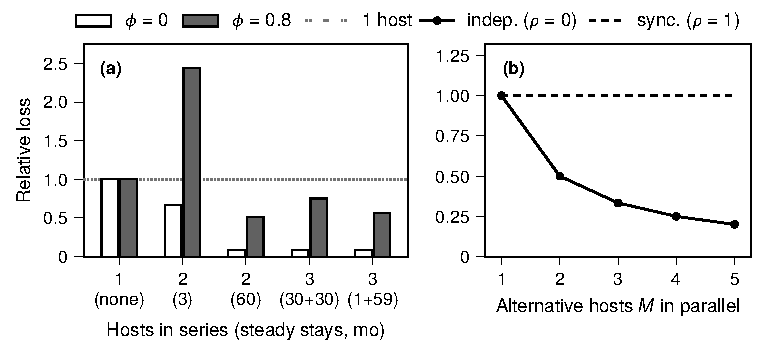
\includegraphics[width=129mm]{figures/example-1.pdf}
\caption{Relative second-order fluctuation loss across illustrative life cycles (parameters as in Table~\ref{tab:example}). Panel~(a) compares one, two, and three obligate hosts in series with a $6$-month fluctuating stay and the indicated steady stays (in months) under uncorrelated ($\phi = 0$, open bars) and autocorrelated ($\phi = 0.8$, shaded bars) host abundance, relative to one host (gray dotted line at $1.0$, $\Gamma/\sigma^2 = 1/12$). Panel~(b) compares $M = 1$ to $5$ equal-share matched alternative hosts in parallel at fixed mean total transfer in a $(6, 24)$-month cycle at $\phi = 0.8$ when cross-host correlation $\rho$ (under Proposition~\ref{prop:ring-alt}) is independent ($\rho = 0$, solid curve with markers) or perfectly synchronous ($\rho = 1$, black dashed line)}\label{fig:example-1}
\end{figure}

First, the number of obligate hosts in series does not decide the outcome. With two hosts in sequence at $\phi = 0.8$, adding a $3$-month steady stay raises the fluctuation loss to $2.44$ times the one-host value, whereas a $60$-month steady stay lowers it to $0.51$ (Table~\ref{tab:example}, Part~A, Fig.~\ref{fig:example-1}a). Time spent in the sheltered stage, rather than host count, governs whether a second host amplifies or halves the penalty (Proposition~\ref{prop:ring-steady}(c), Eq.~\eqref{eq:ring-steady}).

Second, without host memory ($\phi = 0$), only total time outside the fluctuating transfer matters. The second-order loss reduces to $\Gamma = \sigma^2/(2\mathcal{T})$ (Propositions~\ref{prop:ring-band} and~\ref{prop:ring-steady}(b)), so the two-host cycle with a $60$-month steady stay and both three-host cycles ($30 + 30$ and $1 + 59$ months) share $\mathcal{T} = 66$ months and the same relative loss of $0.091$ ($\Gamma/\sigma^2 = 0.00758$). For independent gamma hosts, a one-step exposed stage, and a geometric steady stay, exact threshold loss likewise decreases strictly with steady-stay duration at every fixed positive variance, although that exact benchmark does not cover the $6$-month exposed stage used here (Section~\ref{sec:exact}, Theorem~\ref{thm:exact-mono}).

Third, when host fluctuations carry memory ($\phi > 0$), how sheltered time is divided across stages changes the loss, whereas compartment labels alone do not. At $\phi = 0.8$ and $\mathcal{T} = 66$ months, splitting $60$ sheltered months into $30 + 30$ raises the relative loss from $0.51$ to $0.75$, whereas $1 + 59$ gives $0.57$ (Table~\ref{tab:example}, Part~A, Fig.~\ref{fig:example-1}a). Dividing a sheltered stay into equal substages raises the loss under memory (Proposition~\ref{prop:mech-renewal}), and at fixed $n$ and $\mathcal{T}$ the loss lies between the values for $n - 1$ unit stays and for equal stays (Proposition~\ref{prop:ring-band}, Eq.~\eqref{eq:ring-gamma}). Here, relabeling the two unchanged steady compartments as one host or two leaves the matrix identical. More generally, equal complete sheltered kernels and unchanged exposed dynamics preserve growth and threshold (Section~\ref{sec:mech}, Lemma~\ref{lem:mech-kernel}).

Fourth, under multi-month boom-and-bust dynamics, a short sheltered stay can make things worse. For a two-stage cycle with fluctuating stay $a$ and steady stay $b$ (Proposition~\ref{prop:ring-steady}(c), Eq.~\eqref{eq:ring-steady}), adding $b$ raises $\Gamma$ above the one-host value whenever $a > 1$ and $b < a(2a - 1)\theta/(a + \theta)$ (Section~\ref{subsec:exact-memory}, Proposition~\ref{prop:exact-mem-ring}, Eq.~\eqref{eq:exact-mem-add}). At $a = 6$ and $\theta = 4$ months, $b = 26$ gives relative loss $1.01$ and $b = 27$ gives $0.98$, so a sheltered stay (a ``safe zone'') helps only once it exceeds this threshold (here $26.4$ months, more than six times the memory scale $\theta$).

Fifth, at fixed mean total transfer, equal shares of alternative hosts with matched log variance and memory used in parallel at the fluctuating step divide that step's second-order loss by their number when they fluctuate independently, whereas partial synchrony weakens this reduction, perfect synchrony gives no reduction, and a much noisier newcomer can raise the loss. Replacing one fluctuating host in a $(6, 24)$-month cycle by one to five such equal-share hosts ($M = 1$ to $5$) multiplies the loss by $[1 + \rho(M - 1)]/M$ when cross-covariances at every lag equal $\rho$ times the common autocovariance, giving $1/M$ ($0.50$ at $M = 2$ and $0.20$ at $M = 5$) at $\rho = 0$ and $1.00$ at $\rho = 1$ at both $\phi = 0.8$ and $\phi = 0$ (Table~\ref{tab:example}, Part~B, Fig.~\ref{fig:example-1}b, Proposition~\ref{prop:ring-alt}). In contrast, equal shares of independent hosts with variances $\sigma^2$ and $9\sigma^2$ and matched memory multiply the loss by $2.5$ (Proposition~\ref{prop:ring-alt}, with the general $\phi = 0$ newcomer inequality in Proposition~\ref{prop:mech-routes}, Eq.~\eqref{eq:mech-newcomer}).

Direct simulation of the exact threshold loss $D$ at $\sigma = 0.3$ (600 replicates, at least 20{,}000 months each) for the 18 cases listed in note~b gave values slightly above the quadratic predictions (by $0.0001$--$0.0008$, largest standard error $0.00027$) and ranked the cases as the formulas do, with formula ties reproduced within simulation error (Table~\ref{tab:example}, Eq.~\eqref{eq:model-loss}). The following sections prove these statements in general and show where they stop holding.
